%%% ==========================================================================
%%%  APPENDIX — all supplementary content consolidated here.
%%%  Sections are loaded in order: Threats → Cross-Arch → Reproducibility.
%%% ==========================================================================

% ---------------------------------------------------------------------------
\section{Threats to Validity}
\label{sec:threats}
% ---------------------------------------------------------------------------

\textbf{Construct validity.}
Our primary metric, library efficiency, measures DSL performance relative to the strongest library baseline we were able to exercise for each kernel. Because cuBLAS and cuDNN select among multiple internal algorithms, any failure to invoke their best-performing configuration would make the DSL appear closer to library performance than it actually is. To reduce this risk, we use library-backed PyTorch paths consistent with standard practice, invoke \texttt{cudnnFind} for convolution, record the selected algorithms, and allow cuBLAS to use a large workspace.
We report under default cuDNN flags (no explicit \texttt{cudnn.benchmark} toggle, no NHWC conversion); convolutions run in the PyTorch-default NCHW layout, and algorithm-selection variance is bounded by \texttt{cudnnFind} defaults.

\textbf{Internal validity.}
Profiling-based analysis may be affected by measurement noise and tool overhead. We mitigate this threat by separating end-to-end timing from counter collection, using repeated runs for both, and verifying that key Nsight Compute measurements remain stable across repetitions. All experiments are executed in isolation on a fixed software and hardware setup to reduce confounding effects from concurrent workloads or environmental variation. Locked-clock re-timing (graphics 1215 MHz / memory 1215 MHz) over 100 runs shows run-to-run relative std-dev of 0.0--0.9\% on near-parity kernels, so the reported gaps are statistically significant rather than artifacts of frequency variation.

\textbf{Auto-tuning shape sensitivity.}
Our auto-tuning sweep selects each kernel's configuration by timing the candidate grid at a fixed per-kernel shape that, for several kernels, is smaller than the large deployment shape used for benchmarking.
At the smaller shape the candidates often fall within measurement noise, so the selected configuration can be effectively arbitrary and is occasionally slower than the implementation's hardcoded default at the deployment shape (we observed Triton \texttt{mean\_reduction} at $+136\%$ and \texttt{batched\_matmul} at $+54\%$ relative to the default).
We re-tuned the kernels where this occurred (\texttt{batched\_matmul}, \texttt{mean\_reduction}, and \texttt{attention} in Triton) at the deployment shape, restoring configurations at or below the default ($1.3$--$3.0\times$ faster than the small-shape selection); this touches only those auto-tuned rows and does not affect the reported root causes or heuristics.

\textbf{External validity.}
Our study covers 22 kernels across five operator categories, but it does not represent the full design space of GPU workloads. In particular, the evaluated configurations emphasize common deep learning operators and shapes rather than uncommon cases such as highly dilated convolutions, extreme group counts, or very small batches. Conv2d is evaluated across 1$\times$1, 3$\times$3, 5$\times$5, 7$\times$7, depthwise, and strided variants; the original submission tabulated only 3$\times$3 stride-1.
In addition, our primary measurements span two architectures---the A100-SXM4-40GB (Ampere, sm\_80) and the GH200 (Grace Hopper, sm\_90)---with further cross-architecture replay on the A100-PCIE-40GB (same sm\_80, a form-factor robustness check) and H100-80GB-HBM3 (a cross-family generalization check); results on other vendor backends may still differ.

\textbf{Conclusion validity.}
Our root-cause claims are based on a combination of performance measurements, hardware-counter evidence, and targeted mitigations. Although the mitigation results strengthen the causal interpretation, they do not rule out additional compiler or runtime factors that were not isolated in this study. The conclusions should therefore be read as evidence-supported explanations for the observed gaps, rather than as an exhaustive account of all possible causes.

\textbf{The suite is a probe, not a proposed benchmark.}
Our 22-kernel suite is deliberately not offered as a comprehensive performance benchmark---a central claim of this work (\cref{sec:evaluation}) is that such a benchmark is combinatorially infeasible to build and maintain. The suite instead functions as a diagnostic \emph{probe}: it is large enough to expose the evaluation gap (correct kernels that existing benchmarks admit yet run far below the library), to root-cause that gap across operator classes, and to validate the proposed heuristics, but it is not intended to certify any kernel as production-ready. The contribution is the evaluation methodology---the passes-but-slow demonstration, the authoring/code-generation/library-maturity taxonomy, and the comparability-plus-roofline heuristics---rather than the suite's size.

\textbf{Heuristic assumptions.}
The roofline anchor depends on an essential-work model (bytes moved or FLOPs) and an assumed hardware peak for each kernel; mis-estimating either shifts the achieved fraction $\rho$, and the two checks disagree in a judgment band near $\rho\approx0.5$ (\cref{sec:mitig:heuristics}). We therefore use $\rho$ as a decision signal alongside the comparability screen rather than as a precise efficiency figure, and we record the peak assumptions with each measurement (\cref{tab:roofline}). The suite magnitude is measured on the A100 and the evaluation-gap and roofline results on the GH200---two primary architectures carrying complementary evidence---with per-architecture magnitudes reported where they differ.


% ---------------------------------------------------------------------------
\section{Cross-Architecture Generalization}
\label{sec:xarch}
% ---------------------------------------------------------------------------

The main-paper tables report results on the two primary architectures (A100-SXM4 and GH200).
As a robustness check, we replay the kernel suite and the root-cause taxonomy along an A100-SXM4 / A100-PCIE / H100 axis: the A100-SXM4 serves as the anchor, the A100-PCIE-40GB is a same-architecture (\texttt{sm\_80}) form-factor control, and the H100-80GB-HBM3 is a cross-family (\texttt{sm\_90}) control. The GH200 primary results remain in the main-paper tables.

\Cref{fig:overview:gh200} shows the per-category library-efficiency distribution on the GH200,
parallel to \Cref{fig:overview} in the main paper.
The qualitative profile shifts in two ways: TileLang convolution recovers substantially
(small-shape 8.3\% and large-shape 59.9\% vs.\ A100's 4.1\% and 12.6\%),
while TileLang normalization remains collapsed (LayerNorm 0.3\%), confirming that
the normalization gap is an authoring artifact independent of architecture, whereas
the convolution gap is partly Ampere-specific (\Cref{sec:analysis}).

\begin{figure}[t]
  \centering
  \IfFileExists{figures/overview_efficiency_gh200.pdf}{%
    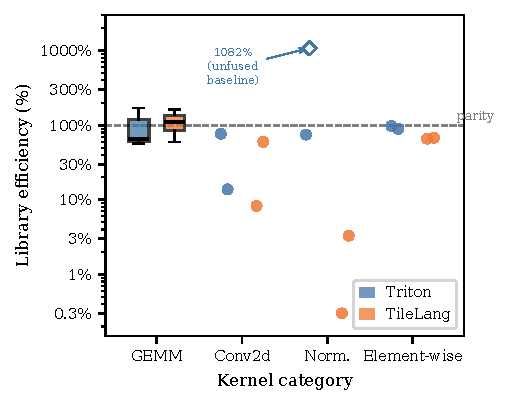
\includegraphics[width=\linewidth]{figures/overview_efficiency_gh200.pdf}%
  }{%
    \fbox{\parbox[c][6cm][c]{\linewidth}{\centering
      \textit{[Figure: GH200 library efficiency (\%) by kernel category and DSL.
      Generate with \texttt{python3 figures/gen\_overview\_gh200.py}.]}}}%
  }
  \caption{Library efficiency (\%) of Triton and TileLang kernels relative to cuBLAS/cuDNN
    on the NVIDIA GH200-480GB, by kernel category (log scale; dashed line = 100\% parity).
    Same layout as \Cref{fig:overview}: GEMM shows IQR boxes; other categories show per-kernel dots.
    $\diamond$~1082\% (Triton, Norm.) marks \texttt{rms\_norm}: unfair-baseline artifact, not a DSL win.
    TileLang Conv2d recovers relative to the A100 (59.9\% large vs.\ 12.6\%);
    TileLang Norm.\ remains collapsed (0.3\%).
    Attention excluded (\Cref{sec:eval:gemm}).}
  \label{fig:overview:gh200}
\end{figure}

% Numbers AUTO-GENERATED by experiments/results/cross_arch/gen_cross_arch_tables.py — do NOT hand-edit.

\begin{table}[t]
  \centering
  \caption{\textbf{Cross-architecture generalization.} Median library efficiency $E_\text{lib}$ (\%) per
    kernel category for each DSL on the primary A100-SXM4 (sm\_80) and the cross-architecture replays
    A100-PCIE (sm\_80, form factor) and H100 (sm\_90, Hopper), untuned defaults. The qualitative
    profile is preserved across architectures: GEMM and element-wise competitive, convolution and
    TileLang normalization severely behind.}
  \label{tab:xarch:summary}
  \resizebox{\columnwidth}{!}{
  \begin{tabular}{lccc@{\hskip 10pt}ccc}
    \toprule
    & \multicolumn{3}{c}{Triton} & \multicolumn{3}{c}{TileLang} \\
    \cmidrule(lr){2-4}\cmidrule(lr){5-7}
    Category & SXM4 & PCIE & H100 & SXM4 & PCIE & H100 \\
    \midrule
    GEMM & 77.3\% & 75.5\% & 68.4\% & 69.4\% & 60.3\% & 69.2\% \\
    Convolution & 31.6\% & 38.0\% & 37.7\% & 9.5\% & 11.1\% & 7.8\% \\
    Normalization & 121.5\% & 137.3\% & 130.5\% & 1.0\% & 0.8\% & 0.9\% \\
    Element-wise/Reduction & 65.3\% & 73.0\% & 72.9\% & 51.0\% & 55.3\% & 60.9\% \\
    \bottomrule
  \end{tabular}}
\end{table}

\begin{table}[t]
  \centering
  \caption{\textbf{Root-cause taxonomy reproduces across architectures.} Each corrected root cause
    measured on all three GPUs with the identical portable harness. All reproduce, confirming they
    are properties of the DSL/compiler rather than of a single GPU (cf.\ \cref{tab:xarch:summary}).}
  \label{tab:xarch:rootcause}
  \resizebox{\columnwidth}{!}{
  \begin{tabular}{lcccl}
    \toprule
    Root cause & SXM4 & PCIE & H100 & Reproduces \\
    \midrule
    RC0 TileLang LayerNorm anomaly ($8192^2$) $E_\text{lib}$ & 0.09\% & 0.09\% & 0.08\% & yes (memory-latency bound) \\
    RC3 Triton conv register spill ($n_\text{spills}$) & 0 & 0 & 0 & yes (no spill; occupancy-bound) \\
    RC4 Winograd upper-bound contribution & 0.1\% & 2.0\% & 20.7\%\textsuperscript{\dag} & yes ($\sim$0--2\%, not primary) \\
    FP32 \texttt{T.gemm} TF32 lowering (rel.\ err) & 633$\times$ & 633$\times$ & 1268$\times$ & yes (TF32 mantissa class) \\
    \bottomrule
  \end{tabular}}
  {\footnotesize \textsuperscript{\dag}~The cuDNN deterministic-mode (Winograd-off) timing on H100 is high-variance ($\sigma\!\approx\!27\%$ of median, un-locked clocks),
    so its determinism A/B over-states the Winograd upper bound; the stable, locked-clock A100-SXM4
    and A100-PCIE measurements bound the Winograd contribution at ${\le}2\%$.}
\end{table}

\begin{table}[t]
  \centering
  \caption{\textbf{GEMM autotuning recovery generalizes (RC2).} Triton matmul $E_\text{lib}$ before
    (plain, heuristic) and after (expanded autotune search) on all three GPUs. The \S5-vs-\S7.3 gap
    is a search-space artifact on every architecture, not shape- or hardware-specific.}
  \label{tab:xarch:autotune}
  \resizebox{\columnwidth}{!}{
  \begin{tabular}{lccc@{\hskip 10pt}ccc}
    \toprule
    & \multicolumn{3}{c}{Triton plain} & \multicolumn{3}{c}{Triton autotuned} \\
    \cmidrule(lr){2-4}\cmidrule(lr){5-7}
    Shape & SXM4 & PCIE & H100 & SXM4 & PCIE & H100 \\
    \midrule
    $4096^2$ & 56.4\% & 57.7\% & 43.2\% & 76.5\% & 110.1\% & 33.1\% \\
    $16384^2$ & 32.5\% & 38.3\% & 33.6\% & 81.8\% & 87.5\% & 70.2\% \\
    \bottomrule
  \end{tabular}}
  {\footnotesize At the RQ1 $16384^2$ shape, expanded autotuning recovers Triton on all three GPUs
    (plain$\to$autotuned). The sub-millisecond $4096^2$ cells on the un-locked PCIE/H100 replays carry
    higher relative noise; the locked-clock A100-SXM4 primary is the reference measurement.}
\end{table}

\begin{table}[t]
  \centering
  \caption{\textbf{Convolution filter sweep across architectures} (large shape $32{\times}256{\times}128^2$,
    groups$=$1, stride$=$1). Triton $E_\text{lib}$ vs cuDNN for each GPU, with the measured Triton
    register-spill count. The gap widening with filter size and the absence of register spilling both
    hold across architectures.}
  \label{tab:xarch:conv}
  \begin{tabular}{lcccc}
    \toprule
    & \multicolumn{3}{c}{Triton $E_\text{lib}$} & Triton \\
    \cmidrule(lr){2-4}
    Filter & SXM4 & PCIE & H100 & $n_\text{spills}$ \\
    \midrule
    $1\times1$ & 28.7\% & 37.0\% & 24.7\% & 0 \\
    $3\times3$ & 19.3\% & 24.4\% & 11.4\% & 0 \\
    $5\times5$ & 13.7\% & 16.9\% & 13.4\% & 0 \\
    $7\times7$ & 9.8\% & 12.5\% & 15.7\% & 0 \\
    \bottomrule
  \end{tabular}
\end{table}


% ---------------------------------------------------------------------------
\section{Reproducibility Details}
\label{app:repro}
% ---------------------------------------------------------------------------

\subsection{Kernel Suite Provenance}
\label{app:repro:kernels}

\paragraph{Selection criteria}
We narrow the candidates from TritonBench~\cite{li2025tritonbench} and the TileLang example repository~\cite{wang2025tilelang} using four criteria applied in order.
\emph{(i) Forward-pass only}: backward and gradient kernels are excluded, as they are governed by different access patterns and reduction structures.
\emph{(ii) Stable library baseline}: each kernel must admit a well-defined cuBLAS, cuDNN, or PyTorch eager reference that computes the same function, making library efficiency a meaningful quantity.
\emph{(iii) Five-category coverage}: we retain kernels that populate the five operator categories (GEMM, attention, convolution, normalization, element-wise/reduction) rather than over-sampling any single class.
\emph{(iv) Canonical operators}: kernels with sparse inputs or runtime-dependent output shapes are excluded for lacking a stable baseline.

\paragraph{Per-kernel provenance}
\Cref{tab:provenance} lists all 22 kernels.
Triton implementations are drawn from TritonBench except \texttt{layer\_norm}, which follows the TorchInductor reference implementation.
All TileLang implementations are our re-implementations of the same operators.
PyTorch implementations are cuBLAS, cuDNN, or PyTorch-eager baselines as described in \cref{app:repro:baselines}.

\begin{table}[h]
  \centering
  \caption{Per-kernel provenance for the 22-kernel ViperBench suite.}
  \label{tab:provenance}
  \resizebox{\columnwidth}{!}{%
  \begin{tabular}{llll}
    \toprule
    Kernel & Category & Triton Source & TileLang Source \\
    \midrule
    \texttt{matmul}             & GEMM          & TritonBench         & Custom \\
    \texttt{batched\_matmul}    & GEMM          & TritonBench         & Custom \\
    \texttt{linear\_activation} & GEMM          & TritonBench         & Custom \\
    \midrule
    \texttt{attention}          & Attention     & TritonBench         & Custom \\
    \midrule
    \texttt{conv2d}             & Convolution   & TritonBench         & Custom \\
    \midrule
    \texttt{layer\_norm}        & Normalization & TorchInductor ref.  & Custom \\
    \texttt{rms\_norm}          & Normalization & TritonBench         & Custom \\
    \midrule
    \texttt{add}                & EW / Red.     & TritonBench         & Custom \\
    \texttt{mul}                & EW / Red.     & TritonBench         & Custom \\
    \texttt{relu}               & EW / Red.     & TritonBench         & Custom \\
    \texttt{leaky\_relu}        & EW / Red.     & TritonBench         & Custom \\
    \texttt{softmax}            & EW / Red.     & TritonBench         & Custom \\
    \texttt{log\_softmax}       & EW / Red.     & TritonBench         & Custom \\
    \texttt{logsumexp}          & EW / Red.     & TritonBench         & Custom \\
    \texttt{swiglu}             & EW / Red.     & TritonBench         & Custom \\
    \texttt{argmax}             & EW / Red.     & TritonBench         & Custom \\
    \texttt{max\_reduction}     & EW / Red.     & TritonBench         & Custom \\
    \texttt{mean\_reduction}    & EW / Red.     & TritonBench         & Custom \\
    \texttt{cross\_entropy}     & EW / Red.     & TritonBench         & Custom \\
    \texttt{matrix\_transpose}  & EW / Red.     & TritonBench         & Custom \\
    \texttt{index\_select}      & EW / Red.     & TritonBench         & Custom \\
    \texttt{embedding}          & EW / Red.     & TritonBench         & Custom \\
    \bottomrule
  \end{tabular}}
  \smallskip
  \begin{minipage}{\columnwidth}
    \small ``Custom'' denotes our re-implementation of the operator following the same interface as
    the TritonBench version; ``TorchInductor ref.''\ denotes an implementation modelled on the
    TorchInductor generated reference for that op.
    EW / Red.\ = element-wise or reduction.
  \end{minipage}
\end{table}


\subsection{Baseline Specifications}
\label{app:repro:baselines}

GEMM baselines use cuBLAS via \texttt{torch.matmul}.
Convolution baselines use PyTorch \texttt{nn.Conv2d} with default NCHW memory layout under standard cuDNN algorithm selection.
Normalization baselines use \texttt{F.layer\_norm} and \texttt{F.rms\_norm}.
Element-wise and reduction baselines use standard PyTorch eager execution.
For attention, we use PyTorch scaled dot-product attention with the FlashAttention backend enabled through \texttt{enable\_flash\_sdp(True)}.

\paragraph{GEMM notation and exclusions}
Per-shape GEMM latencies are in the artifact (\texttt{slow\_kernels.csv}); $16384^2$ denotes a square $16384\times16384$ FP16 GEMM and $64\times128^2$ a batched GEMM of batch 64 over $128\times128$ matrices.
FP32 TileLang GEMM is excluded: \texttt{T.gemm} silently lowers to TF32, making FP32 results a precision artifact rather than a logic error (\Cref{sec:analysis:jit}).
\Cref{tab:summary} reports the category medians; the $16384^2$ Triton slowdown to 32.8\% reflects an under-populated auto-tune search space (RC2), while TileLang reaches 80.0\% on that shape via an explicit schedule.


\subsection{Measurement Protocol}
\label{app:repro:meas}

\paragraph{End-to-end timing}
We measure host-synchronized GPU execution time using \texttt{time.perf\_counter()} bracketed by \texttt{torch.cuda.synchronize()} calls.
Each measurement uses 10 warm-up iterations followed by 100 timed iterations; we report the median.
Results reflect GPU-side execution only, excluding host-side dispatch overhead, and each workload runs in isolation.

\paragraph{Clock-lock settings}
On the A100-SXM4-40GB, we pin graphics and memory clocks to 1215\,MHz and 1215\,MHz respectively via \texttt{nvidia-smi --lock-gpu-clocks} and \texttt{--lock-memory-clocks}.
The nominal maximum is 1410\,MHz, but that setting power-caps under the 400\,W board limit and causes clock throttling; 1215\,MHz is stable and yields run-to-run relative standard deviation of 0.0--0.9\% across 100-iteration timing windows.
On the GH200, clocks are locked at 1320\,MHz (graphics) and 2619\,MHz (memory).

\paragraph{Nsight Compute counter definitions}
We collect the following seven counters per kernel; each is gathered from a single \texttt{ncu} execution and verified within 2\% across five repeats.

\begin{enumerate}
  \item \textbf{Global-load efficiency} --- fraction of global memory transactions that serve requested bytes (1.0 = perfectly coalesced).
  \item \textbf{Sectors per request} --- average number of L1/L2 cache sectors accessed per memory instruction; lower values indicate better coalescing.
  \item \textbf{Registers per thread} --- register file allocation per thread; high values increase occupancy pressure and can trigger spill.
  \item \textbf{Register spills} --- bytes spilled from the register file to thread-local memory (L1/L2/DRAM); non-zero values denote register-pressure-induced latency.
  \item \textbf{Long-scoreboard stall cycles} --- warp stall cycles waiting for L2 or DRAM data; the dominant stall for memory-bound kernels.
  \item \textbf{Barrier stall cycles} --- warp stall cycles at thread-block synchronization barriers (\texttt{\_\_syncthreads} / \texttt{bar.sync}).
  \item \textbf{L2 sector hit rate} --- fraction of L2 cache sector accesses that hit; low rates indicate DRAM pressure.
\end{enumerate}

\paragraph{KernelBench evaluator harness}
For the passes-but-slow demonstration (\cref{sec:eval:passesslow}), we invoke KernelBench's \texttt{eval\_kernel\_against\_ref} function, which (i) overrides the candidate kernel's \texttt{get\_inputs} and \texttt{get\_init\_inputs} with those of the reference implementation so input shapes cannot be altered by the candidate, (ii) checks output equivalence on randomized inputs at the same per-dtype tolerances as our correctness suite (\cref{sec:meth:profiling}), and (iii) emits a warning only if the candidate's throughput exceeds $10\times$ the reference---a speedup-only guard that admits any slowdown.
We record pass/fail and measure slowdown separately using our clock-locked timing harness.


\subsection{Full Hardware and Software Stack}
\label{app:repro:stack}

\paragraph{Hardware}

\begin{table}[h]
  \centering
  \caption{GPU hardware specifications for the two primary architectures.}
  \label{tab:hw:specs}
  \resizebox{\columnwidth}{!}{%
  \begin{tabular}{lll}
    \toprule
    Property & A100-SXM4-40GB & GH200 \\
    \midrule
    Architecture      & Ampere (\texttt{sm\_80}) & Grace Hopper (\texttt{sm\_90}) \\
    SMs               & 108                      & 132 \\
    Memory            & 40\,GB HBM2e             & 96\,GB HBM3 \\
    Peak mem.\ BW     & $\sim$1.5\,TB/s          & $\sim$4.0\,TB/s \\
    Peak FP16 TC      & $\sim$312\,TFLOP/s       & $\sim$989.5\,TFLOP/s \\
    L2 cache          & 40\,MB                   & 60\,MB \\
    TDP               & 400\,W                   & 900\,W (SoC) \\
    Clock lock (g/m)  & 1215 / 1215\,MHz         & 1320 / 2619\,MHz \\
    NVIDIA Driver     & 610.43.02                & --- \\
    CUDA Toolkit      & 12.8                     & 12.8 \\
    \bottomrule
  \end{tabular}}
\end{table}

\paragraph{Software stack}

\begin{table}[h]
  \centering
  \caption{Pinned software versions for all experiments.}
  \label{tab:sw:stack}
  \begin{tabular}{ll}
    \toprule
    Package & Version \\
    \midrule
    PyTorch        & 2.8.0+cu128 \\
    Triton         & 3.4.0 \\
    TileLang       & 0.1.6.post1 \\
    cuDNN          & bundled with PyTorch \\
    Nsight Compute & 2026.2.0 \\
    \bottomrule
  \end{tabular}
\end{table}

All experiments use default cuDNN algorithm selection flags and pre-warm the Triton auto-tuner before measurement.
A complete \texttt{requirements.txt} and \texttt{environment.yaml} pinning all transitive dependencies are distributed with the artifact.
